\documentclass[twocolumn]{article}
\usepackage{hyperref}
\usepackage{graphicx}
\graphicspath{ {./} }

\begin{document}
\title{\textbf{BibTrek: A Graph Visualization Tool for Cybersecurity Research Publications}}
\date{}
\author{Jos\'{e} Eduardo Br\'{a}s\\Instituto Superior T\'{e}cnico, Universidade de Lisboa, Portugal}
\date{July 2019}
\maketitle

\textbf{\textit{Abstract}--With the advent of more elaborate cyberattacks, security researchers and operators are having difficulty in keeping up with the lasted research results. In many occasions, it is not trivial to discover the most important paper regarding one topic. The technical information is usually present in scientific research publications and most of the knowledge present in them relies on the work of several other publications, which they reference. To assist in this research and study endeavor, we propose BibTrek, a tool that can query bibliographic APIs and store data in a graph than can be visualized. With BibTrek we make use of several computer science web-based libraries to acquire information from multiple sources and display them into a graph database to better relate the references between publications, but also authors and other relevant information. We present the implementation of a prototype that reads data from DBLP and stores the results in the Neo4J database. The code is available on GitHub.}

\section{Introduction}

The number of cyberattacks is on the rise. The CVE statistics \cite{cvestatisticsbyyear} show an average increase of 21.56\% in the number of documented vulnerabilities over the past 19 years. With the amount of information available it is very easy for an ill-intentioned individual to carry out an attack and exploit some system with minimal computacional resources. 
\\[1\baselineskip]
As a result of the rising number of cyberattacks, it is becoming hard to find white-hat hackers that know how to thwart attacks effectively. However, with the increased availability of information on the web it is becoming easier to study and learn how attacks work. The techniques used to carry them out are are mostly found in blog posts and other social media with short publication times. However, for in-depth analysis and scientific rigour of fundamental problems, there are scientific publications in peer-reviewed conferences and journals. Due to the many iterations of scientific knowledge the most recent work builds upon the work that has been done on the past. Because of this, to understand the most recent concepts it is important to read the referenced papers that made the writing of the current ones possible. Usually the most cited papers are the most relevant regarding a certain subject. Having said that, the reality is that performing these kinds of bibliography surveys is time-consuming and inefficient, thus, there is a opportunity for improvement.

\subsection{Solution}
The visualization of information using graphs has the potential to improve the learning process and the construction of conceptual mind maps that make it easier to retain information and relate it with other topics \cite{enhancinglearningwithvisualizationtechniques}. With BibTrek we propose a graph visualization tool with the goal of relating the many different research papers in the area of cybersecurity and presenting that in an informative and easy-to-browse graph. The use of this result is therefore useful to relate the papers and their references making the survey process more efficient. We implemented a tool prototype that allows a search from a set of either authors, publication titles or keywords dynamically producing a reference graph composed of the most relevant scientific papers allowing an easier navigation of information. 

\subsection{Example}
A simple example execution would follow these steps. Let us say we want to learn about the \emph{Spectre} attack on microprocessors. We would choose the option to query one of the mentioned above libraries. Next, by selecting the option to search for a publication, we would then type the word ``Spectre'' on the console terminal. After choosing a publication, the paper its references, authors and its subject will be added to the database and related with the other papers that were previously added by the user. After the fact, the user can simply watch the graph visualization created by BibTrek, this way finding which papers are the most referenced and therefore understand which shall be the one that he should read first.


\subsection{Overview}
In section 2 we present the solution design and implementation. In section 3 we present an evaluation of the results and functionalities of BibTrek. In section 4 we show related work from other authors. In section 5 we discuss further developments to the application. Finally, in section 6 we present a brief conclusion of the work. \\[1\baselineskip]


\section{Solution}

In this section we present the design and implementation of the BibTrek prototype. Here we discuss the use of the software that was used for the design of the application and the reasoning behind its choice. We also go in depth about the specifics of the implementation including the communication protocol, data parsing, access and storage.

\subsection{Design}
To obtain the required information to populate our graph database we make use of the APIs provided to us by the major computer science libraries that host scientific research publications. After searching what the appropriate libraries were given their terms of service and API functionalities we have chosen the libraries of ArXiV, DBLP and IEEEXplore \cite{arxiv, dblp, ieeexplore}. We present the results of the surveyed publicly-available bibliographic APIs in Table 1. ``Crawlers'' is related with the permission for using a bot to crawl the information available in the webpage. The ``API'' column mentions if the library has an available remote invocation service for the developer to use. Finally the ``Key'' column mentions the requirement of a special key to access the API. \\[1\baselineskip]
Our app is presented through a simple command line Java program that receives user provided queries, crawls the libraries mentioned above using their APIs and adds to the Neo4j\cite{neo4j} graph database all the available information about either publications, institutions, authors and subjects. This graph database can also later be queried through the use of console commands to infer useful information about the bibliography.\\[1\baselineskip]
The BibTrek application was written using the Java programming language mainly due to the fact that it is ubiquitous on modern-day computing systems. The database module uses Neo4j and requires us to have either a local or remote instance running it. The connection of the JVM to the Neo4j is made using the BOLT protocol on network port 7687. The JSON format was chosen as the way to retrieve the information from the DBLP database using the API due to it being lightweight and having overall great flexibility. The Neo4j database is queried using Cypher\cite{cypher} which is its standard query language. The application was built using the Apache Maven tool and uses the Neo4j driver and JSON maven repositories. Finally, we use the java.net package in order to establish an HTTP connection with the DBLP API.

\begin{table}[]
\captionof{\textbf{Table 1 - Publicly available bibliographic APIs}}
\\[1\baselineskip]
\begin{tabular}{c|c|c|c|}
\cline{2-4}
\multicolumn{1}{l|}{}                     & API & Crawlers & Key \\ \hline
\multicolumn{1}{|c|}{ACM Digital Library} & No  & No       & N/A \\ \hline
\multicolumn{1}{|c|}{ArXiV}               & Yes & Yes      & No  \\ \hline
\multicolumn{1}{|c|}{DBLP}                & Yes & Yes      & No  \\ \hline
\multicolumn{1}{|c|}{Google Scholar}      & No  & No       & N/A \\ \hline
\multicolumn{1}{|c|}{IEEEXplore}          & Yes & No       & Yes \\ \hline
\end{tabular}
\end{table}

\subsection{Operation}
At the present time, BibTrek only uses the information obtained from querying DBLP API to populate our server. In the current implementation after choosing one of the available options to query the database, the user inputs either an author's name or publication title that is  parsed into a query. Queries are done through the composition of a specifically formatted URL link and an HTTP request. After the query is successfully processed by the DBLP database the JSON response is parsed and displayed in the terminal console. Afterwards the user will choose from the available publications that were displayed on the console which are the ones that he would like to add to Neo4J database. These publications which are encoded in the JSON format are transformed into a Cypher query and written into a file. This file will later be used to create nodes and the relationships between them in our Neo4j database. This file is processed by a thread that periodically searches the current folder for newly written update files and is responsible for storing this information into the graph database. Once the thread has finished its update these files are then moved to a different folder not to be re-written into the database. \\[1\baselineskip]
An example execution of a query would be the following. The user starts by choosing the option to query the libraries for a publication by its title. Let us say he chose to query the system for publications about the \emph{Spectre} attack. Because of this a query is properly formatted in the following way: \url{https://dblp.org/search/publ/api/?q=Spectre&format=json}. The ``q=Spectre`` parameter in the URL link meaning that we are querying the system for Spectre subject; ``search/publ/api/`` means we will be using its API and search for a publication; ``&format=json`` means we want the fetched data in the JSON format. After obtaining the HTTP response and parsing its JSON the information is then displayed to the user. Here, all the found publications about the Spectre attack is shown on the console, for the user to choose one or more of them, adding them to the Neo4j database. Afterwards, the chosen information is then parsed into a Cypher query and stored. The thread responsible for the Neo4j communication and data storage will search the BibTrek file system for newly added files. If a new file is found the most recent data is then stored in the Neo4j database. The Neo4j Java thread moves the most recently written file to a different folder than the one mentioned before. Finally, the constructed graph can then be observed using the Neo4j browser by the user and infer useful information about the Spectre attack its authors and other related papers.

\begin{figure}[t]
\centering
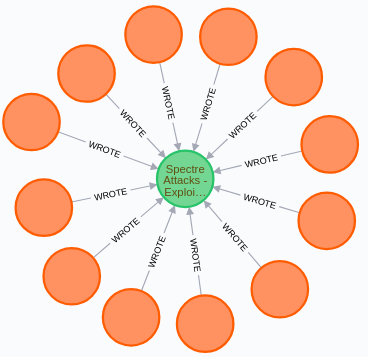
\includegraphics[scale=0.55]{spectre.png}
\caption{Illustration of the display for the Spectre publication.}
\end{figure}

\subsection{Command-line interface}
Here we present a more detailed functioning of the user interface. We show the available options for the user to interact with, and explain the way the system interacts with the web based library.
\\[1\baselineskip]
Once the application is started we are presented with the choice of either selecting the option to query the DBLP database or exit the program. Once the first is chosen, it is presented to us the available options to query the database. These options are the following:

\begin{itemize}
\item \textbf{Query by author}. Choosing it, we are required to type the name of the author we want to search. Afterwards BibTrek fetches all authors present in the DBLP database with a similar name to the one that we have inserted previously. We are then told to pick which of the fetched authors we want to insert into the database.
\item \textbf{Query by publication's title.}. Here, we type the title of the publication we want to find. After querying DBLP, we are presented with all the available publications bearing a similar title. We are then required to pick which of the displayed publications we want to add to our local database.
\item \textbf{Query by author publications}. Similar to the first option, we type the author's name. BibTrek then fetches us all the available authors in the system. We are then asked to choose which of the retrieved authors we want to search publications of. After doing so, the system fetches us all the available publications for the chosen authors incrementally. Finally, we are required to choose which of the displayed publications we want to insert into the system
\end{itemize}
Any given step of the above procedures we can choose either the option of adding all the displayed information to our data set or exit the current state of the system.

\section{Evaluation}
In this section we discuss the tests that were done using the application to query a web based library and the parsing and processing of the results. Furthermore we elaborate on the functionalities present in the BibTrek prototype. Finally, we list the commands available on the program's terminal console.

\\[1\baselineskip]
We have tested our application for a set of author and publication queries whilst locally running Neo4j using a computer with the following hardware specifications:
\begin{itemize}
\item \textbf{OS:} 64-bit Ubuntu 18.04.2 LTS GNU/Linux 
\item \textbf{CPU:} Intel Core 2 Duo P8700 @ 2.534GHz 
\item \textbf{GPU:} Intel Mobile 4 Series Chipset
\item \textbf{RAM:} 4096MB @ 1066Mhz 
\end{itemize}
BibTrek successfully processed and inserted all nodes and relations into the Neo4j database. We were able to search for any added data with ease. However, the data retrieved from the DBLP database might present a variable number of field attributes. Since we are following a fixed attribute structure for our node data, some of these fields are ignored. Future versions should consider adding these fields dynamically, we further these considerations on the Future Work section of this article.

\section{Related Work}
Some similar work has been done using both graph databases and an interwined network of publications' references. This work is briefly analyzed below.\\[1\baselineskip]
\textbf{Cross Ref} \cite{crossref} is a platform on which the registered publishers are given the option to store and relate their publication references with other available database publications. BibTrek stores publications as nodes in the database and relates every available node through their references. While Cross Ref does not visually represent its data, BibTrek does so using a graph database, also, differently to Cross Ref, is given to us the option to add user input publications that have been dynamically fetched from different libraries.\\[1\baselineskip]
\textbf{VIS - Google Scholar Citation Visualisation} \cite{vis} is an application that is used to create a graph based on a geographic map that has information about a publication, for example, the place where it has been written, relating it, like BibTrek, through its references and citations with other publications all over the said map. While BibTrek does not use a map representation, on the other hand, unlike VIS, that only uses Google Scholar, BibTrek uses different libraries to fetch its information from. Finally, BibTrek is more versatile given the fact that it does not base its graph around a single publication, but every node that has been added to the system by the user so far. \\[1\baselineskip]
\textbf{Book recommendation using Neo4j graph database in BibTeX book metadata} \cite{bookrecusingneo4j} is an application that uses BibTeX metadata from books to build a Neo4j graph representation, through the use of user input Cypher queries, about either the author's name or book type, can recommend books. Similarly to BibTrek, a Neo4j graph representation is used after parsing a book's metadata. The main difference compared to BibTrek is the focus around authors, keywords, publications and subjects whilst this application being focused exclusively on books. Finally, Cypher queries are similarly done but to fetch the most referenced paper given a single author, keyword or publication title, making the scope different from book searching alone.

\section{Future Work}
The current version of this project was developed in one person-month. Because of this there are many aspects of the current BibTrek implementation that can be further engineered and developed. To begin data can be fetched from more than one web based library. At the current moment only the DBLP is being used. The ArXiV API is free to use, IEEE Xplore requires the use of a key attributed to its developers, but should also be usable. Another aspect that should be considered is the use of dynamic attributes since, at the moment, any block of data that is fetched has some of its attributes unused because, we adhere to a fixed attribute schema when adding data to the database. In the current version the nodes being added to the database are either Authors or Publications. We should consider adding Companies, Universities and other Institutions that authors are or have been linked with in the past, Keywords/Subjects and any other relevant information for the user. The BibTrek data schema should be developed to be able to represent a ``union'' of the most popular bibliographic databases. Furthermore, in the current version BibTrek allows the user to add duplicated information. \\[1\baselineskip]
Another key aspect to develop is the ability to infer better relations between the nodes already stored in the database. With this point in mind, we could use the node's URL attribute to download the publication's PDF and use a text reading tool such as iText in order to read its references and through them relate which node references each. This way we can have a richer graph and understand which of the papers is the most important building block to learn about a certain subject. Again, information that is trying to be added must be compared with the one that has been put there already. Finally, we are not able to query our Neo4j graph database through the terminal console, apart from the example module, since there was not enough time to implement it in the current version of the system. The work to be done regarding this topic, is the development of querying the database through a user input choice from specific functions that manipulate the information present there, displaying relevant information about the current status of the data to the user we the intent on aiding its research process. An example of a query would be getting the most referenced paper by all the papers presently on the database with respect to a certain subject.

\section{Conclusion}
This paper describes the BibTrek prototype that was implemented. It allows us to query the DBLP database and acquire diverse information. Currently it presents a functional user interface. BibTrek's main potential is the simplification of an exploratory bibliographic database to our advantage. This way we would be able to add even more data and create a very complex but informative graph. There is also some work to be done in inferring more information than the one being currently inferred about the retrieved data from DBLP, adding more nodes and attributes to the graph representation.

\section*{Acknowledgements}
The writer of this article would like to thank Professor Miguel L. Pardal and INESC-ID for having invited him for a one month summer-internship program and for the reviewing of this article.

\begin{thebibliography}{9}

\bibitem{arxiv}
arXiv 2019,
\textit{arXiv API | arXiv e-print repository},
arXiv, viewed 29 July 2019,
\url{https://arxiv.org/help/api}

\bibitem{crossref}
Crossref 2019,
\textit{You are Crossref - Crossref},
Crossref, viewed 29 July 2019,
\url{https://www.crossref.org/}

\bibitem{cvestatisticsbyyear}
CVE 2019,
\textit{Browse cve vulnerabilities by date - CVE Details},
CVE, viewed 30 July 2019,
\url{https://www.cvedetails.com/browse-by-date.php}

\bibitem{bookrecusingneo4j}
I. N. P. W. Dharmawan and R. Sarno, 
\textit{Book recommendation using Neo4j graph database in BibTeX book metadata}, 2017.
In: 3rd International Conference on Science in Information Technology (ICSITech). 
Bandung, Indonesia.

\bibitem{cypher}
Neo4j 2019,
\textit{Cypher Query Language - Neo4j},
Neo4j, viewed 29 July 2019,
\url{https://neo4j.com/developer/cypher-query-language/}

\bibitem{dblp}
dblp 2019,
\textit{How to use the dblp search API? - dblp},
dblp, viewed 29 July 2019,
\url{https://dblp.uni-trier.de/faq/How+to+use+the+dblp+search+API}

\bibitem{ieeexplore}
IEEE Xplore 2019,
\textit{IEEE Xplore API},
IEEE Xplore, viewed 29 July 2019,
\url{https://developer.ieee.org}

\bibitem{enhancinglearningwithvisualizationtechniques} 
J. Klerkx, K. Verbert, E. Duval,
\textit{Learning with Visualization Techniques}, 2014.
In: J. Spector, M. Merrill, J. Elen, M. Bishop 
\textit{Handbook of Research on Educational Communications and Technology}. 
Springer, New York, New York.

\bibitem{neo4j} 
Neo4j 2019, 
\textit{Neo4j Graph Platform – The Leader in Graph Databases}, 
Neo4j, viewed 29 July 2019, 
\url{https://neo4j.com}

\bibitem{vis}
C. Yang, I. Todd, L. Sanby, 2019,
\textit{Google Scholar Citation Visualisation},
Google Scholar Citation Visualisation, viewed 29 July 2019,
\url{https://people.cs.uct.ac.za/~yngcha005/vis2015/index.html}


\end{thebibliography}

\end{document}